\documentclass[10pt]{beamer}

\usetheme{default}

\usepackage[utf8]{inputenc}
\usepackage[russian]{babel}
\usepackage[OT1]{fontenc}
\usepackage{amsmath}
\usepackage{amsfonts}
\usepackage{amssymb}
\usepackage{graphicx}
\usepackage{etoolbox}
\usepackage{caption}
\usepackage{subcaption}
\usepackage{pifont}
\usepackage{xcolor}
\usepackage{framed}
\definecolor{shadecolor}{cmyk}{0,0,0,1}
\usepackage{listings}

\lstset{
	backgroundcolor=\color{lightgray},
	commentstyle=\color{blue},
	frame=single
	breakatwhitespace, 
	language=python, 
	columns=fullflexible, 
	keepspaces, 
	breaklines, 
	tabsize=3, 
	showstringspaces=false, 
	extendedchars=true,
	numbers=left
}

\makeatletter

\setbeamercolor{title}{fg=white}
\setbeamercolor{frametitle}{fg=black}
\setbeamerfont*{title}{family=\sffamily,size=\LARGE}

\setbeamerfont{page number in head/foot}{size=\scriptsize}
\setbeamertemplate{footline}[frame number]
\let\otp\titlepage
\renewcommand{\titlepage}{\otp\addtocounter{framenumber}{-1}}

\setbeamertemplate{background canvas}{%
	\ifnumequal{\c@framenumber}{0}{%
      
\includegraphics[width=\paperwidth,height=\paperheight]{images/cover.png}
   }{%
      \ifnumequal{\c@framenumber}{\inserttotalframenumber}{
         
\includegraphics[width=\paperwidth,height=\paperheight]{images/back.png}
      }{%
         % Other frames
      }%
   }%
}

\makeatother

\beamertemplatenavigationsymbolsempty

\author{Николай Анохин}
\title{\newline \newline \newline Лекция 4 \\ Визуализация результатов кластеризации}

\begin{document}

\begin{frame}[plain]
\titlepage
\end{frame}

\begin{frame}{Краткое содержание предыдущих лекций}

{\bf Дано.} $N$ обучающих $D$-мерных объектов $\mathbf{x}_i \in \mathcal{X}$, образующих тренировочный набор данных (training data set) $X$.

\vspace{1em}
{\bf Найти.} Модель $h^*(\mathbf{x})$ из семейства параметрических функций $H = \{h(\mathbf{x, \mathbf{\theta}}): \mathcal{X} \times \Theta \rightarrow \mathbb{N}\}$, ставящую в соответствие произвольному $\mathbf{x} \in \mathcal{X}$ один из $K$ кластеров так, чтобы объекты внутри одного кластера были похожи, а объекты из разных кластеров различались.

\end{frame}

\begin{frame}{Краткое содержание предыдущей лекции}

\begin{columns}[C]
    \begin{column}{.4\textwidth}
    	Рассмотрели классические алгоритмы кластеризации
		\begin{enumerate}
			\item Смесь гауссовских распределений и k-means
			\item Hierarchical Clustering
			\item DBSCAN
		\end{enumerate}    	
    \end{column}
       
    \begin{column}{.6\textwidth}
    \vspace{-0em}
	\begin{center}
   		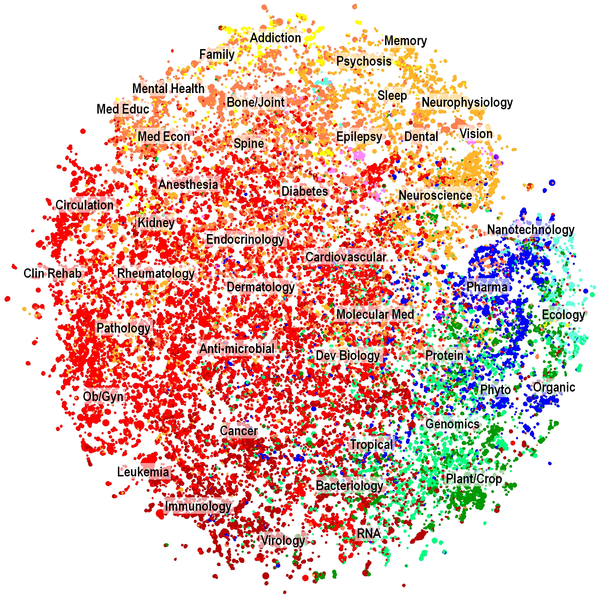
\includegraphics[width=\textwidth]{images/medical.png}
    \end{center}
    \end{column}
  \end{columns}

\end{frame}

% ============================================== %

\section{Multidimensional Scaling}

% ============================================== %

\begin{frame}

\begin{center}
{\Large Multidimensional Scaling}
\end{center}

\end{frame}

\begin{frame}{Идея метода}

Перейти в пространство меньшей размерности так, чтобы расстояния между объектами в новом пространстве были подобны расстояниям в исходном пространстве.

\end{frame}

\begin{frame}{Обозначения}

\begin{itemize}
\item $\mathbf{x}_i \in \mathcal{X} \subset R^D$ -- объекты в исходном многомерном пространстве
\item $\delta_{ij}$ -- расстояние между $\mathbf{x}_i$ и $\mathbf{x}_j$
\item $\mathbf{x}_i \in \mathcal{Y} \subset R^E$ -- объекты в целевом пространстве ($E=2$ или $E=3$)
\item $d_{ij}$ -- расстояние между $\mathbf{y}_i$ и $\mathbf{y}_j$
\end{itemize}

\begin{center}
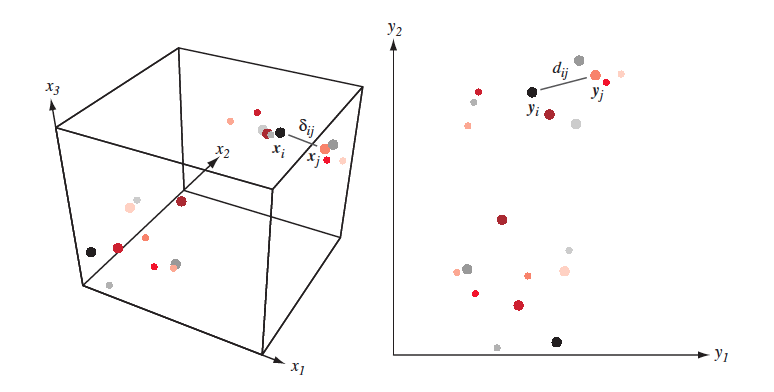
\includegraphics[scale=0.35]{images/mds.png}
\end{center}

\end{frame}

\begin{frame}{Критерии}

Выбираем кофигурацию $\mathbf{y}_i$, соответствующую минимуму критерия
\begin{itemize}
\item \[
J_{ee} = \frac{\sum_{i < j} (d_{ij} - \delta_{ij})^2} {\sum_{i < j} \delta_{ij}^2}
\]
\item \[
J_{ff} = \sum_{i < j} \frac{(d_{ij} - \delta_{ij})^2}{\delta_{ij}^2}
\]
\item \[
J_{ef} = \frac{1} {\sum_{i < j} \delta_{ij}}\sum_{i < j} \frac{(d_{ij} - \delta_{ij})^2}{\delta_{ij}}
\]
\end{itemize}

\end{frame}

\begin{frame}

\begin{itemize}
\item \[
\nabla_{\mathbf{y}_k}J_{ee} = \frac{2} {\sum_{i < j} \delta_{ij}^2} \sum_{j \neq k} (d_{kj} - \delta_{kj}) \frac{\mathbf{y}_k - \mathbf{y}_j}{d_{kj}}
\]
\item \[
\nabla_{\mathbf{y}_k} J_{ff} = 2 \sum_{j \neq k} \frac{d_{kj} - \delta_{kj}}{\delta_{kj}^2} \frac{\mathbf{y}_k - \mathbf{y}_j}{d_{kj}}
\]
\item \[
\nabla_{\mathbf{y}_k} J_{ef} = \frac{2} {\sum_{i < j} \delta_{ij}} \sum_{j \neq k} \frac{d_{kj} - \delta_{kj}}{\delta_{kj}} \frac{\mathbf{y}_k - \mathbf{y}_j}{d_{kj}}
\]
\end{itemize}

\end{frame}

% ============================================== %

\section{T-SNE}

% ============================================== %

\begin{frame}

\begin{center}
{\Large T-SNE}
\end{center}

\end{frame}

\begin{frame}[plain]
\begin{center}
{\Large Вопросы}
\end{center}
\end{frame}

\end{document}